\documentclass[11pt,a4paper]{amsart}
\usepackage[T1]{fontenc}
\usepackage{lmodern}
\usepackage{amssymb}
\usepackage{microtype}
\usepackage{booktabs}
\usepackage{graphicx}
\usepackage[hyphens]{url}
\usepackage[colorlinks=true,linkcolor=black,citecolor=black,urlcolor=black]{hyperref}
\usepackage[margin=2.5cm]{geometry}

\hypersetup{
  pdftitle={Measurable density bounds hold for all colourings of the plane with algebraic forbidden distances},
  pdfauthor={Sergi Gal\'an},
  pdfsubject={The Hadwiger-Nelson problem},
  pdfkeywords={Hadwiger-Nelson problem, chromatic number of the plane, forbidden distances, fractional chromatic
  number, distance-avoiding sets, linear programming}}

\newtheorem{theorem}{Theorem}
\newtheorem{corollary}[theorem]{Corollary}
\newtheorem{lemma}[theorem]{Lemma}
\newtheorem{proposition}[theorem]{Proposition}
\theoremstyle{definition}
\newtheorem{definition}[theorem]{Definition}
\theoremstyle{remark}
\newtheorem*{remark}{Remark}

\newcommand{\C}{\mathbb{C}}
\newcommand{\Q}{\mathbb{Q}}
\newcommand{\R}{\mathbb{R}}
\newcommand{\Z}{\mathbb{Z}}
\newcommand{\N}{\mathbb{N}}
\newcommand{\E}{\mathbb{E}}
\newcommand{\dens}{\overline{\delta}}
\newcommand{\chif}{\chi_{\mathrm f}}

\title[Density bounds for all colourings of the plane]{Measurable density bounds hold for all colourings of the
plane with algebraic forbidden distances}
\author{Sergi Gal\'an}
\thanks{These results were obtained with the assistance of an AI system (Claude, by Anthropic), which found the
observation, wrote the programs, ran the checks and helped to draft this note. Five separate AI agents refereed
the note with their own programs. The hard input is OpenAI's transfer theorem \cite{OpenAI}. No mathematician has
checked the note yet. The author is not a professional mathematician and submits it for independent verification.}
\date{Draft, version 7, 10 October 2026}
\subjclass[2020]{Primary 05C15, 52C10; Secondary 05C72, 42B10, 90C05}
\keywords{Hadwiger--Nelson problem, chromatic number of the plane, forbidden distances, fractional chromatic number,
distance-avoiding sets, linear programming bounds}

\begin{document}

\begin{abstract}
OpenAI recently proved that every colouring of the plane with five colours gives the same colour to two points at
distance $1$. The proof transfers an arbitrary proper colouring of the plane to a \emph{weak measurable} one, and then
excludes weak measurable $5$-colourings. We observe that the transfer works, with the same proof, for every set of
algebraic forbidden distances and for fractional colourings. Upper bounds for the density of measurable sets avoiding
given distances therefore become lower bounds for arbitrary colourings; all these lower bounds rest on OpenAI's
rigidity theorem, which OpenAI formalized in Lean; we formalized the transfer for proper colourings (not its
fractional version) on top of their formalization. Consequences: the fractional chromatic number
of the plane equals $1/m_1(\R^2)$, where $m_1(\R^2)$ is the largest density of a measurable planar set with no two
points at distance $1$, so it lies between $4.0485$ and $4.36$; and the least independence ratio of an $n$-point
unit-distance graph tends to $m_1(\R^2)$, as conjectured by Dúcz and Varga. If the distances $1$ and $2$ are both
forbidden, at least $7$ colours are needed, improving the bound $6$ of Exoo and Ismailescu; the same holds for
$\{1,\sqrt3\}$, and at least $8$, $10$, $11$ and $13$ colours are needed for $\{1,11/6\}$, $\{1,40\}$,
$\{1,100\}$ and $\{1,1000\}$. Uniformly in $d$, $\chi(\R^2,\{1,d\})\ge7$ for every real algebraic $d\ge5.82$ and for
$1.72\le d\le2.04$, and the bound rises step by step to $14$ for every real algebraic $d\ge25\,700$; each step is
proved by a single certificate for a whole half-line of $d$, using unit equilateral triangles and Moser spindles. The
distances $1$, $100$ and $10^4$ force $27$ colours, $1$, $10$, $100$ and $1000$ force $26$, and $1$, $30$, $900$ and
$27000$ force $48$. For
suitable sets of $k$ integer distances more than $4.0485^k$ colours are needed, in the plane and in every higher
dimension, so the
chromatic number with $k$ forbidden distances grows exponentially in $k$, whereas Erd\H{o}s expected polynomial
growth. Davies has just proved the analogous statements in dimension at least $4$ by a different method. Using OpenAI's
theorem itself at a small scale and density bounds at a large one, we show that the distances $1$ and $N$ force at
least $25$ colours for every large algebraic $N$, although $19.01$ colours suffice fractionally, and, with de
Grey's graph, at least $18$ colours for every algebraic $N\ge10^{25}$; iterating, $k$ distances can force at least
$6\cdot4.0486^{k-1}$ colours. The density
bounds we use are linear-programming bounds of Oliveira Filho and Vallentin, which we certify in interval arithmetic,
and theorems of Bukh and of Ambrus, Csiszárik, Matolcsi, Varga and Zsámboki.
\end{abstract}

\maketitle

\section{Results}

For a set $D$ of positive real numbers, $\chi(\R^2,D)$ is the least number of colours needed to colour the plane so
that no two points whose distance lies in $D$ get the same colour. The Hadwiger--Nelson problem is the case
$D=\{1\}$; OpenAI \cite{OpenAI} proved $\chi(\R^2)\ge 6$, and $\chi(\R^2)\le 7$ is Isbell's hexagonal colouring
\cite{Soifer}. For two distances $\{1,d\}$ the best known lower bound was $6$: Owings, Tetiva and Huddleston
\cite{OTH} showed $\chi(\R^2,\{1,(1+\sqrt5)/2\})\ge6$ (as reported in \cite{CJW,DeNeve}), Exoo and Ismailescu
\cite{EI} proved $\chi(\R^2,\{1,2\})\ge 6$, Parts \cite{Parts} gave a small $6$-chromatic two-distance graph, and De
Neve, Vanden Kerchove, Colle, Tavernier and Pickavet \cite{DeNeve} gave $6$-chromatic graphs for $d=\sqrt3$ and
$d=(\sqrt6+\sqrt2)/2$, two cases claimed earlier in the Polymath16 project \cite{Polymath}; Chybowska-Sokół, Junosza-Szaniawski and Węsek \cite{CJW}
record as open whether some pair $\{1,d\}$ forces $7$ colours.

OpenAI's proof has two steps. Their Theorem~1.3 (the transfer) says that the plane has a proper $k$-colouring if and
only if it has a \emph{weak measurable} $k$-colouring: a measurable colouring in which the pairs of points at distance
$1$ with the same colour have measure zero. Their Theorem~1.4 excludes weak measurable $5$-colourings. The transfer
rests on a rigidity theorem for invariant measures on the character group of the algebraic plane
\cite[Thm.~2.3]{OpenAI}. Its proof uses neither that the forbidden distance is $1$ nor that a colouring uses finitely
many colours rather than being fractional. We record the two generalisations (Theorems~\ref{thm:A}
and~\ref{thm:B}) and their consequences.

Write $m_D(\R^2)$ for the supremum of the upper densities of measurable sets $A\subseteq\R^2$ with no two points at a
distance in $D$, and $m_1(\R^2)=m_{\{1\}}(\R^2)$. Croft's construction gives $m_1(\R^2)\ge 0.229364$ \cite{Croft},
and Ambrus, Csiszárik, Matolcsi, Varga and Zsámboki \cite{ACMVZ} proved $m_1(\R^2)\le 0.2470$, confirming a
conjecture of Erd\H{o}s that $m_1(\R^2)<1/4$. For the fractional chromatic number we use two versions, defined in
Section~\ref{sec:notation}: the finitary one $\chi_{\mathrm f,0}(\R^2,D)$, the supremum over finite graphs drawn in
the plane with edge lengths in $D$, and the fractional chromatic number $\chif(\R^2,D)$ of the whole infinite graph.

\begin{theorem}\label{thm:main}
Let $D$ be a finite set of positive real algebraic numbers. Then
\[
\chi(\R^2,D)\;\ge\;\chi_{\mathrm f,0}(\R^2,D)\;=\;\chif(\R^2,D)\;=\;\frac1{m_D(\R^2)}.
\]
\end{theorem}

The lower bound $\chi_{\mathrm f,0}(\R^2,D)\ge1/m_D(\R^2)$, and with it every lower bound below, rests on OpenAI's
rigidity theorem \cite[Thm.~2.3]{OpenAI}, which OpenAI formalized in Lean; the upper bound
$\chif(\R^2,D)\le1/m_D(\R^2)$ is elementary.

\subsection*{One distance}

\begin{corollary}\label{cor:frac}
$\chi_{\mathrm f,0}(\R^2)=\chif(\R^2)=1/m_1(\R^2)$, and $4.0485<1/0.2470\le\chif(\R^2)\le 1/0.229364<4.36$.
\end{corollary}

The constants in \cite[§8]{ACMVZ} give $m_1(\R^2)<0.2469975$, hence $\chif(\R^2)>4.0486$. Matolcsi, Ruzsa, Varga and
Zsámboki \cite{MRVZ} proved $\chif(\R^2)\ge 4$ and conjectured that $\chi_{\mathrm f,0}(\R^2)=4$ and that
$\chif(G)<4$ for every finite unit-distance graph $G$ \cite[Conj.~1]{MRVZ}; the value $4$ had also been conjectured
in \cite[Remark after Cor.~2]{ACMVZ}. Dúcz and Varga \cite{DV} disproved this conjecture: they found a unit-distance
graph $G_{29}$ whose geometric fractional chromatic number exceeds $4.0007$, which gives a finite unit-distance graph
with independence ratio below $1/4$ and $\chif(\R^2)>4.0007$. Corollary~\ref{cor:frac} gives a second disproof and
determines $\chif(\R^2)$ in terms of $m_1(\R^2)$. It also answers the question of \cite{MRVZ} whether
$\chi_{\mathrm f,0}(\R^2)=\chif(\R^2)$, and with \cite[Thm.~2]{MRVZ} it shows that the finitary independence ratio
of the plane equals the measurable one, which \cite{MRVZ} remark would fail if their conjecture held. Let $f(n)$ be
the least independence number of the unit-distance graph of a set of $n$ points in the plane, the function of
Erd\H{o}s's question \cite{Erdos87} answered by Dúcz and Varga.

\begin{corollary}\label{cor:ratio}
$f(n)\ge m_1(\R^2)\,n$ for every $n$, and $f(n)/n\to m_1(\R^2)$ as $n\to\infty$. In particular $f(n)<0.2470\,n$ for
all large $n$.
\end{corollary}

The first statement is the classical averaging bound $m_1(\R^2)\le\alpha_1(\R^2)$ \cite[Remark after
Cor.~2]{ACMVZ}, \cite[(14)]{MRVZ}, \cite[Claim~1]{DV}; the new content is the limit, that is,
$\alpha_1(\R^2)=m_1(\R^2)$. Dúcz and Varga conjectured that $f(n)/n=m_1(\R^2)+o(1)$, and in particular that
$m_1(\R^2)$ is the density
$0.2293647\ldots$ of Croft's construction \cite[Conj.~1]{DV}. Corollary~\ref{cor:ratio} proves the first statement;
the second remains open.

\subsection*{Two distances}

\begin{corollary}\label{cor:two}
\begin{gather*}
\chi(\R^2,\{1,2\})\ge 7,\qquad \chi(\R^2,\{1,\sqrt3\})\ge 7,\qquad
\chi\bigl(\R^2,\{1,(\sqrt6+\sqrt2)/2\}\bigr)\ge 7,\\
\chi(\R^2,\{1,11/6\})\ge 8,\qquad \chi(\R^2,\{1,40\})\ge 9,\\
\chi(\R^2,\{1,100\})\ge 10,\qquad \chi(\R^2,\{1,1000\})\ge 12.
\end{gather*}
Moreover $\chi(\R^2,\{1,d\})\ge 17$ for every sufficiently large real algebraic number $d$.
\end{corollary}

The finite bounds come from linear programs certified in Section~\ref{sec:lp}, and the last statement from Bukh's
theorem \cite{Bukh}; products of hexagonal colourings give $\chi(\R^2,\{1,d\})\le49$. For \emph{measurable}
colourings, bounds of this kind were known: Oliveira Filho and Vallentin \cite[§4]{OFV} report, from their linear
program, the bound $0.141577<1/7$ for the density of a measurable set avoiding the distances $1$ and
$j_{1,2}/j_{1,1}\approx1.8309$, a ratio of zeros of $J_1$, and, combining Bukh's theorem with their bound for
$m_1(\R^2)$, they show $\inf_{d_1,d_2}m_{\{d_1,d_2\}}(\R^2)\le m_1(\R^2)^2\le0.072046$; so pairs of distances whose
density is close to $m_1(\R^2)^2$ need $14$ colours for measurable colourings ($17$ with the bound of
\cite{ACMVZ}). What is new here is that such bounds hold for arbitrary colourings; the bounds for $\{1,2\}$ and
$\{1,\sqrt3\}$, which use clique inequalities, also seem to be new for measurable colourings.

The same linear program gives bounds for whole ranges of $d$ at once.

\begin{theorem}\label{thm:uniform}
Let $d\ge1$ be a real algebraic number and $7\le k\le14$. Then $\chi(\R^2,\{1,d\})\ge k$ whenever $d\ge d_k$, where
\begin{gather*}
d_7=5.82,\quad d_8=10.5,\quad d_9=18.9,\quad d_{10}=35.7,\quad d_{11}=73.6,\\
d_{12}=181,\quad d_{13}=655,\quad d_{14}=25\,700.
\end{gather*}
Moreover $\chi(\R^2,\{1,d\})\ge7$ for $1.72\le d\le2.04$, and $\chi(\R^2,\{1,d\})\ge8$ for $1.82\le d\le1.89$. The
same bounds hold for $\chi(\R^2,\{1,1/d\})=\chi(\R^2,\{1,d\})$, and, for measurable colourings, for every real
$d$.
\end{theorem}

Theorem~\ref{thm:uniform} contains the finite bounds of Corollary~\ref{cor:two} and raises the ones for $\{1,40\}$,
$\{1,100\}$ and $\{1,1000\}$ to $10$, $11$ and $13$; see Figure~\ref{fig:uniform}. Scaling the plane by $1/d$ turns $\{1,d\}$ into $\{1/d,1\}$,
which gives the equality with $1/d$. For measurable colourings neither the transfer nor algebraicity is needed:
Proposition~\ref{prop:lp} and Lemma~\ref{lem:tail} do not use them, and one class of a measurable proper $k$-colouring
avoiding $\{1,d\}$ is a measurable set avoiding $\{1,d\}$ of upper density at least $1/k$. For measurable colourings
bounds of this size were known for one pair \cite[§4]{OFV} and, by Bukh's theorem, for all $d$ beyond an unspecified
threshold (see the discussion after Corollary~\ref{cor:two}); there the new content is the explicit thresholds and
ranges. For each $k$ a single function serves every $d\ge d_k$ (Lemma~\ref{lem:tail} and Table~\ref{tab:uniform}),
and each of the two bounded ranges is covered by finitely many functions, each serving an interval of $d$
(Section~\ref{sec:uniform}). All of them use the clique inequalities of unit equilateral triangles, the tails also
the inequalities of Moser spindles (Proposition~\ref{prop:lp} with $\alpha=2$, as in \cite{KMOR}), and the thresholds
are close to the best this method can give: in floating point, the program of Lemma~\ref{lem:tail} gives $k$ colours
from about $d=5.797$, $10.42$, $18.81$, $35.53$, $73.36$, $179.5$, $652.6$ and $25\,590$ on, for $k=7,\dots,14$. Without spindles it gives $7,\dots,13$ colours from about $5.800$,
$10.67$, $20.04$, $40.04$, $90.24$, $261.7$ and $1544$ on and never $14$; without triangles and spindles, from about
$6.503$, $12.03$, $23.87$, $52.85$, $139.9$, $599.2$ and, for $k=13$, from somewhere between $50\,000$ and
$54\,300$. For a single $d$ the program with triangles is below $1/6$, for $1<d<5.8$,
only for $d$ between about $1.716$ and $2.045$ and from about $5.55$ on. As $d\to\infty$ the value of the program
without cliques tends to $\mu_0^2/(1+\mu_0)^2=1/12.13\ldots$, where $\mu_0=-\min J_0=0.40275\ldots$: the square of
its value $\mu_0/(1+\mu_0)=0.287119$ for one distance \cite[§3.2]{OFV} (Remark after Lemma~\ref{lem:tail}). With
triangles and spindles its floating-point value at $D=10^7$ is $0.075778=1/13.20$, close to the product
$0.075362=1/13.27$ of $0.287119$ and the value $0.262476$ of the one-distance program with our triangles and spindles
(with triangles alone the values are $1/12.80$ and $0.271823$). So, in floating point, these configurations give no
more than $14$ colours for two distances; Theorem~\ref{thm:C} gives more for very large $d$.

\begin{figure}[ht]
\centering
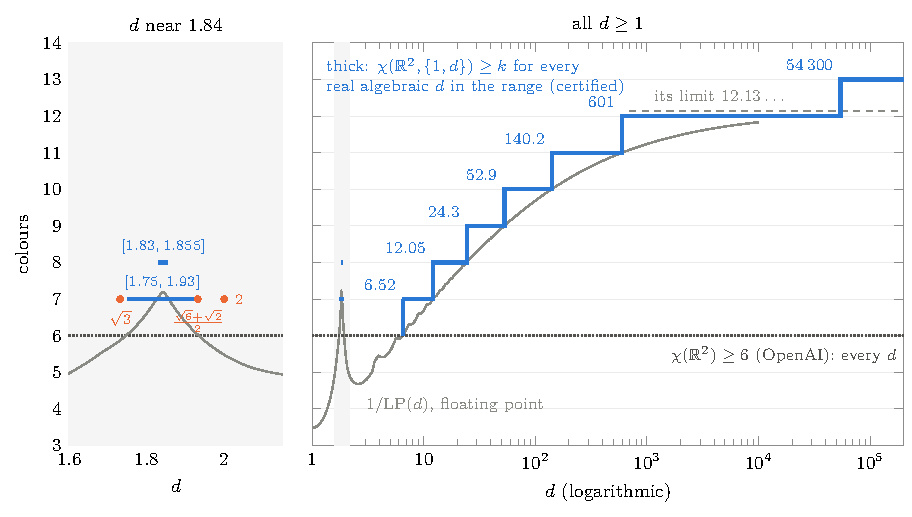
\includegraphics[width=\textwidth]{uniform-bounds}
\caption{Lower bounds for $\chi(\R^2,\{1,d\})$, $d\ge1$; the same hold for $1/d$. Thick blue: Theorem~\ref{thm:uniform},
for every real algebraic $d$ in the range. Orange: the pairs $\{1,\sqrt3\}$, $\{1,2\}$ and $\{1,(\sqrt6+\sqrt2)/2\}$
of Corollary~\ref{cor:two}. Grey, solid: $1/\mathrm{LP}(d)$, where $\mathrm{LP}(d)$ is the value, in floating point
(not a proof), of the linear program for the single distance $d$ with unit-triangle cliques ($d\le6.6$); grey,
dash-dotted: the same for the program of Lemma~\ref{lem:tail} with triangles and spindles, whose value at $D$ serves
every $d\ge D$. A certified bound below $1/(k-1)$ gives $k$ colours, so each blue step lies less than one colour above
the curve it follows. Dashed: the limit $13.27$ of the second program (floating point). Dotted: $\chi(\R^2)\ge6$ \cite{OpenAI}, which
holds for every $d$. Left: the shaded range $1.6\le d\le2.15$ on a linear scale.}
\label{fig:uniform}
\end{figure}

\subsection*{Many distances}

\begin{corollary}\label{cor:many}
For every $k\ge1$ there is a set $D$ of $k$ positive integers with
$\chi(\R^d,D)\ge\chi(\R^2,D)\ge m_1(\R^2)^{-k}>4.0485^k$ for every $d\ge2$. Moreover
\[
\sup\bigl\{\chif(\R^2,D):D\subseteq F\cap(0,\infty),\ |D|=k\bigr\}=m_1(\R^2)^{-k},
\]
where $F$ is the field of real algebraic numbers.
\end{corollary}

Erd\H{o}s \cite{Erdos81} defined $L_2(r)$ as the largest chromatic number of the plane with $r$ forbidden distances
and asked: ``Does $L_2(r)$ increase polynomially or exponentially? I expect that $L_2(r)<r^c$ for some absolute
constant $c$.'' The question is Problem~\#706 on Bloom's list \cite{EP706}, where it is stated for finite point sets,
which gives the same $L_2(r)$ by the de~Bruijn--Erd\H{o}s theorem; Croft, Falconer and Guy ask whether the growth is
exponential \cite[Problem G11]{CFG} (as quoted by Bukh \cite{Bukh}), and the best lower bound in the plane was of order
$k\sqrt{\log k}$ (see \cite{Bukh,Naslund}). By Corollary~\ref{cor:many} and the product colouring,
\[
4.0485^r<L_2(r)\le7^r ,
\]
so $L_2(r)$ grows exponentially, contrary to Erd\H{o}s's expectation. Bukh \cite{Bukh} proved exponential growth for
measurable colourings and remarked that it is ``very likely that the usual chromatic number does not share this
behavior''; Corollary~\ref{cor:many} shows that it does, for integer distances. Davies \cite{Davies} has just proved
exponential growth for arbitrary colourings of $\R^d$, $d\ge4$, with a different transfer (see the Remarks);
Corollary~\ref{cor:many} gives it in every dimension $d\ge2$ (for $d\ge4$ Davies's base $1/m_1(\R^d)$ is
larger, for distances with rational squares). Like all our lower bounds, it rests on
\cite[Thm.~2.3]{OpenAI}. Bukh also conjectured that $\chi(\R^d,D)$ is bounded independently of $D$ when the elements
of $D$ are algebraically independent \cite{Bukh}; Theorem~\ref{thm:A} says nothing about such $D$.

The same linear programs give explicit sets (Table~\ref{tab:many}):

\begin{corollary}\label{cor:explicit}
$\chi(\R^2,\{1,40,1600\})\ge22$, $\chi(\R^2,\{1,10,100,1000\})\ge26$, $\chi(\R^2,\{1,100,10^4\})\ge27$ and
$\chi(\R^2,\{1,30,900,27000\})\ge48$.
\end{corollary}

These numbers are far below $m_1(\R^2)^{-k}$, which is approached only by very spread distances, but the sets are
explicit and the bounds are certified.

\subsection*{Two scales}

The lower bounds so far come from densities alone, so for two distances they never exceed the fractional chromatic
number, which is below $19.01$ for every pair $\{1,N\}$ (Corollary~\ref{cor:scales}). Using OpenAI's theorem itself
at one scale and densities at the other gives more.

\begin{theorem}\label{thm:C}
Let $D_1$ and $D_2$ be finite sets of positive real algebraic numbers, let $c$ be a positive integer with
$c\le\chi(\R^2,D_1)$, and let $W$ be a finite graph drawn in the plane with all edge lengths in $D_2$. There is $N_0$
such that
\[
\chi(\R^2,D_1\cup ND_2)\ \ge\ \chi_c(W)\ \ge\ c\,\chif(W)
\]
for every real algebraic number $N\ge N_0$. Consequently, with $c=\chi(\R^2,D_1)$,
\[
\chi(\R^2,D_1\cup ND_2)\ \ge\ \chi_c(\R^2,D_2)\ \ge\ \frac{c}{m_{D_2}(\R^2)}
\]
for all large real algebraic $N$.
\end{theorem}

Here a \emph{$c$-fold colouring} of a graph with $k$ colours gives every vertex a set of $c$ of the $k$ colours,
with disjoint sets at adjacent vertices, and the $c$-fold chromatic number $\chi_c$ is the least such $k$ (Stahl's
$c$-th chromatic number; see \cite{GJSW} for the plane). So $\chi_1=\chi$, $\chi_c\ge c\,\chif$ for finite graphs,
and $\chi_c(\R^2,D)=\chi_c(G(\C,D))$.

At the scale of $D_1$, every disc of a fixed radius meets at least $c$ classes of the measurable colouring given
by Theorem~\ref{thm:A}, each in a set of measure bounded below, because a finite graph that needs $c$ colours fits in
the disc; at the scale of $ND_2$ these classes behave like a $c$-fold colouring. For graphs, the analogue is Geller
and Stahl's formula $\chi(G[H])=\chi_{\chi(H)}(G)$ for the lexicographic product \cite{GS}, and Theorem~\ref{thm:C}
is the lower half of a geometric version; whether $\chi(\R^2,D_1\cup ND_2)\to\chi_{\chi(\R^2,D_1)}(\R^2,D_2)$ as
$N\to\infty$ is open (products of colourings give only $\chi(\R^2,D_1)\,\chi(\R^2,D_2)$). The proof is in
Section~\ref{sec:scales}. For $c=6$ no explicit finite graph is known, so $N_0$ is not explicit; with explicit inputs
it is (the remark on explicit pairs in Section~\ref{sec:scales}).

\begin{corollary}\label{cor:scales}
\begin{enumerate}
\item $\chi(\R^2,\{1,N\})\ge25$ for every sufficiently large real algebraic number $N$, whereas
$\chif(\R^2,\{1,N\})\le m_1(\R^2)^{-2}<19.01$ for every $N>0$.
\item There are integers $1<d_2<d_3<d_4$ with $\chi(\R^2,\{1,d_2\})\ge25$, $\chi(\R^2,\{1,d_2,d_3\})\ge102$ and
$\chi(\R^2,\{1,d_2,d_3,d_4\})\ge413$, and for every $r\ge1$ there is a set $D$ of $r$ positive integers with
$\chi(\R^d,D)\ge\chi(\R^2,D)\ge6\cdot4.0486^{r-1}$ for every $d\ge2$. Hence $L_2(r)>1.48\cdot4.0486^r$.
\end{enumerate}
\end{corollary}

So for two distances the chromatic number can exceed the fractional chromatic number by a factor above
$25/19.01>1.3$. For a single distance, OpenAI's theorem and Corollary~\ref{cor:frac} give the factor $6/4.36>1.37$.
The bound $6/m_1(\R^2)$ that Theorem~\ref{thm:C} gives for $\{1,N\}$ lies between $24.29$ and $26.16$, while products
of hexagonal colourings give $\chi(\R^2,\{1,N\})\le49$. The bound $25$ needs only some finite unit-distance
graph $W$ with $\chif(W)>4$, such as the graph of Dúcz and Varga \cite{DV}, so it does not depend on
Theorem~\ref{thm:B} or on \cite{ACMVZ}; the constants $102$ and $413$ do (from $\chif(W)>4.0007$ alone one gets
$25$, $101$ and $405$).

None of these results comes with an explicit finite graph: as in \cite{OpenAI}, the finite graphs exist by
compactness.

\section{Notation}\label{sec:notation}

Identify the plane with $\C$. Let $F=\overline{\Q}\cap\R$, let $E=F(i)$ be the plane of algebraic points and
$K=\{u\in E:|u|=1\}$ its group of rotations, as in \cite[Def.~2.1]{OpenAI}. For $D\subseteq(0,\infty)$ and
$X\subseteq\C$ let $G(X,D)$ be the graph on $X$ in which two points are adjacent when their distance lies in $D$. A
set of real algebraic numbers is countable, and for $d\in F$ the points of $E$ at distance $d$ from $0$ are exactly
those of $dK$.

\emph{Fractional chromatic numbers.} For a graph $G$ with countably many vertices, $\chif(G)$ is the least $t$ such
that some Borel probability measure on the closed set of independent sets of $G$ in $\{0,1\}^{V(G)}$ gives every
vertex probability at least $1/t$ of lying in the random set. For finite $G$ this is the usual fractional chromatic
number, and by weak-$*$ compactness $\chif(G)$ is the supremum over the finite subgraphs of $G$. We write
$\chi_{\mathrm f,0}(\R^2,D)$ for the supremum of $\chif(H)$ over finite graphs $H$ drawn in the plane with all edge
lengths in $D$, the \emph{finitary} fractional chromatic number of \cite{MRVZ} when $D=\{1\}$, and $\chif(\R^2,D)$
for the infimum of $\sum_I w(I)$ over finitely supported weightings $w\ge0$ of independent sets of $G(\C,D)$ with
$\sum_{I\ni x}w(I)\ge1$ for every point $x$. Clearly $\chi_{\mathrm f,0}\le\chif$. Since $F$ is real closed,
Tarski's transfer principle lets every finite graph drawn with edge lengths in $D\subseteq F$ be redrawn with
vertices in $E$; so, for $D\subseteq F$,
\[
\chi_{\mathrm f,0}(\R^2,D)=\chif(G(E,D))\quad\text{and}\quad\chi(\R^2,D)=\chi(G(E,D)).
\]

\emph{Densities.} The upper density of a measurable $A\subseteq\C$ is
\[
\dens(A)=\limsup_{R\to\infty}\frac{|A\cap B(0,R)|}{|B(0,R)|}.
\]
A set \emph{avoids} $D$ if no two of its points are at a
distance in $D$, and $m_D(\R^2)$ is the supremum of $\dens(A)$ over measurable sets $A$ avoiding $D$. For finite $D$
it is also the supremum of the densities of periodic sets avoiding $D$ (Lemma~\ref{lem:periodic}; the same proof
works with squares in place of discs), so it does not matter whether densities are taken over discs, as here, or over
squares, as in \cite{OFV,Bukh}. A measurable set $A$
\emph{weakly avoids} $D$ if
\[
\int_{B(0,R)}\int_{S^1}1_A(x)\,1_A(x+du)\,d\sigma(u)\,dx=0\qquad\text{for all }d\in D,\ R>0,
\]
where $\sigma$ is the normalized arc length. A \emph{weak measurable $k$-colouring avoiding $D$} is a measurable map
$c:\C\to\{1,\dots,k\}$ whose classes weakly avoid $D$.

\section{The transfers}\label{sec:transfer}

From \cite{OpenAI} we use Lemma~4.1 (the continuous vectors of a measure-preserving action of $E$ form $L^2$ of a
factor, and the translations extend to a strongly continuous action $T_x$, $x\in\R^2$, on it), Theorem~2.3 (every
$K$-invariant Borel probability measure on the character group of the discrete group $E$ that gives measure zero to
the continuous characters is Haar measure), the measurable sampling step in the proof of Proposition~4.2, and
Lemma~4.3. Lemma~4.1 and Theorem~2.3 involve no distance; Lemma~4.3 and the sampling step concern the unit circle,
and we redo them at radius $d$ (Lemma~\ref{lem:density} and the proofs below).

\begin{lemma}\label{lem:density}
If a measurable set $A$ weakly avoids $D$, then the set $A^*$ of points of density one of $A$ avoids $D$, and
$|A\setminus A^*|=0$.
\end{lemma}

\begin{proof}
This is \cite[Lemma~4.3]{OpenAI} at radius $d$. Let $x,\ y=x+v\in A^*$ with $|v|=d\in D$. For small $h>0$ choose
$x'$ uniformly in $B(x,h)$ and, independently, $v'=du'$ with $u'$ uniform on the arc $\{u\in S^1:|du-v|<h\}$. Then
$P(x'\notin A)\to0$. The point $x'+v'$ is a mixture of uniform points of discs of radius $h$, so it has a density at
most $1/(\pi h^2)$, and it lies in $B(y,2h)$; hence $P(x'+v'\notin A)\le|B(y,2h)\setminus A|/(\pi h^2)\to0$. For
small $h$ both points lie in $A$ with positive probability, while the law of $(x',u')$ is absolutely continuous with
respect to $dx\,d\sigma(u)$. This contradicts weak avoidance. The second statement is Lebesgue's density theorem.
\end{proof}

\begin{theorem}\label{thm:A}
Let $D\subseteq F$ be a set of positive real algebraic numbers and $k\ge1$. If $G(E,D)$ has a proper $k$-colouring,
the plane has a weak measurable $k$-colouring avoiding $D$; conversely, such a colouring gives a proper
$k$-colouring of $G(\C,D)$. In particular $\chi(\R^2,D)\ge 1/m_D(\R^2)$.
\end{theorem}

\begin{proof}
This is the proof of \cite[Thm.~1.3]{OpenAI} with the unit circle replaced by the circles of radii $d\in D$.
\begin{enumerate}
\item Let $\Omega_D\subseteq\{1,\dots,k\}^E$ be the closed set of proper colourings of $G(E,D)$, nonempty by
hypothesis. Translations by $E$ and rotations by $K$ preserve it. The group $E\rtimes K$ is amenable, so averages of a
point mass along a F\o lner sequence have an invariant weak-$*$ limit $\mu$.
\item Let $f_i$ be the indicator that the origin has colour $i$. Properness gives $\langle f_i,T_zf_i\rangle=0$ for
$z\in dK$, $d\in D$.
\item By \cite[Lemma~4.1]{OpenAI}, $f_i=p_i+b_i$ where $p_i$ is the conditional expectation on the factor of
continuous vectors; $0\le p_i\le1$, $\sum_ip_i=1$, both parts are rotation-fixed, and the spectral measure of $b_i$ is
$K$-invariant and null on the continuous characters. By \cite[Thm.~2.3]{OpenAI} it is a multiple of Haar measure, so
$\langle b_i,T_zb_i\rangle=0$ for $z\in E\setminus\{0\}$; the cross terms vanish because the continuous subspace and
its orthogonal complement are translation invariant. Hence $\langle p_i,T_zp_i\rangle=0$ for $z\in dK$.
\item The $T_x$ act strongly continuously and $dK$ is dense in the circle of radius $d$, so
$\langle p_i,T_xp_i\rangle=0$ whenever $|x|\in D$.
\item The sampling step of \cite[Prop.~4.2]{OpenAI} gives jointly measurable fields $H_i(x,\omega)$ representing
$T_xp_i$. Since $D$ is countable, a single sample $\omega$ makes all the integrals
\[
\int_{B(0,m)}\int_{S^1}H_i(x,\omega)H_i(x+du,\omega)\,d\sigma(u)\,dx\qquad(m\in\N,\ d\in D,\ \text{all } i)
\]
vanish and has $\sum_iH_i(x,\omega)=1$ for almost every $x$. Giving $x$ the least $i$ with $H_i(x,\omega)>0$ defines the weak
measurable colouring.
\item Conversely, by Lemma~\ref{lem:density} the density-one points of the classes form disjoint sets avoiding $D$
whose union is conull. Every finite configuration has a translate inside that union, so every finite subgraph of
$G(\C,D)$ is $k$-colourable, and the de~Bruijn--Erd\H{o}s theorem \cite{dBE} gives a proper colouring. One of the $k$
sets has upper density at least $1/k$, so $k\ge 1/m_D(\R^2)$.\qedhere
\end{enumerate}
\end{proof}

\emph{Formal verification.} Theorem~\ref{thm:A}, in the form used in Section~\ref{sec:scales}, is formally verified
in Lean~4 (version 4.34.1, Mathlib commit \texttt{d13f23b7}) on top of OpenAI's formalization of their proof
(\url{https://github.com/openai/math}, commit \texttt{fd4aeeb2}): for every set $D$ of positive real algebraic numbers,
a proper $k$-colouring of $G(\C,D)$ gives a measurable $k$-colouring whose classes weakly avoid every $d\in D$
(\path{OAI.Ext.proper_to_borel_weak_distances}), and $k$ pairwise disjoint measurable sets, each avoiding $D$,
whose union is conull (\path{OAI.Ext.proper_to_measurable_classes}); Lemma~\ref{lem:density} at radius $r$ is
\path{OAI.Ext.weak_density_proper_radius}. The proofs use only the standard axioms (\texttt{propext},
\texttt{Classical.choice}, \texttt{Quot.sound}); the files are in \path{lean/external/openai-five/distances/} of
\cite{Repo}. Not formalized: the converse of Theorem~\ref{thm:A}, the inequality $\chi\ge1/m_D$, Theorem~\ref{thm:B},
the lemmas of Section~\ref{sec:scales} and the density bounds.

\begin{theorem}\label{thm:B}
For every set $D\subseteq F$ of positive real algebraic numbers, $\chi_{\mathrm f,0}(\R^2,D)\ge 1/m_D(\R^2)$.
\end{theorem}

\begin{proof}
Let $t\ge\chi_{\mathrm f,0}(\R^2,D)=\chif(G(E,D))$ and let $P$ be a Borel probability measure on the compact
metrizable space $\Omega$ of independent sets of $G(E,D)$ with $P(z\in I)\ge1/t$ for all $z\in E$. Averaging the
push-forwards of $P$ under $E\rtimes K$ along a F\o lner sequence and taking a weak-$*$ limit gives an invariant
probability $\mu$ with $\mu(0\in I)\ge1/t$, since each push-forward has this property and the event is clopen. Let
$f=1[0\in I]$. It is rotation-fixed, and $\langle f,T_zf\rangle=\mu(0\in I,\ z\in I)=0$ for $z\in dK$, $d\in D$,
because $I$ is independent. Steps 3 and 4 of the proof of Theorem~\ref{thm:A} apply to the single function $f$, with
$\sum_ip_i=1$ (which is used only in Step 5) replaced by $\E_\mu p=\E_\mu f$: for $p=\E(f\mid\text{continuous
factor})$ we get $0\le p\le1$, $\E_\mu p\ge1/t$ and $\langle p,T_xp\rangle=0$ whenever $|x|\in D$.

Take a jointly measurable $H:\C\times\Omega\to[0,1]$ with $H(x,\cdot)=T_xp$ in $L^2(\mu)$ for almost every $x$ (the
sampling step of \cite[Prop.~4.2]{OpenAI}). For $m\in\N$ and $d\in D$,
\[
\int_\Omega\int_{B(0,m)}\int_{S^1}H(x,\omega)H(x+du,\omega)\,d\sigma(u)\,dx\,d\mu(\omega)
=\int_{B(0,m)}\int_{S^1}\langle T_xp,T_{x+du}p\rangle\,d\sigma(u)\,dx=0,
\]
so, $D$ being countable, for $\mu$-almost every $\omega$ all these inner integrals vanish. Let
$X_n(\omega)=|B(0,n)|^{-1}\int_{B(0,n)}H(x,\omega)\,dx\in[0,1]$. Since $\E_\mu H(x,\cdot)=\langle
T_xp,1\rangle=\langle p,1\rangle\ge1/t$ for almost every $x$ ($T_x1=1$ and $T_x$ is unitary), $\E_\mu X_n\ge1/t$,
and the reverse Fatou lemma gives $\E_\mu\limsup_nX_n\ge1/t$. Hence $\limsup_nX_n\ge1/t$ on a set of positive
measure, and we choose $\omega$ in it and in the conull set above. Let $A=\{x:H(x,\omega)>0\}$. Then
$1_A\ge H(\cdot,\omega)$, so $\dens(A)\ge1/t$; and $H(x,\omega)H(x+du,\omega)=0$ for almost every $(x,u)$ gives
$1_A(x)1_A(x+du)=0$ almost everywhere, so $A$ weakly avoids $D$. By Lemma~\ref{lem:density}, $A^*$ avoids $D$ and
$\dens(A^*)\ge1/t$. Hence $m_D(\R^2)\ge1/t$.
\end{proof}

\section{The upper bound and the corollaries}\label{sec:upper}

\begin{lemma}\label{lem:periodic}
Let $D$ be finite, $M=\max D$ and $\varepsilon>0$. There are $\eta>0$ and a periodic set $A'$ with period lattice
$N\Z^2$, each period a finite union of squares, that avoids $D_\eta=D+[-\eta,\eta]$ and has density at least
$m_D(\R^2)-\varepsilon$.
\end{lemma}

\begin{proof}
Let $A$ be measurable, avoiding $D$, with $\dens(A)>m_D-\varepsilon/4$, and fix $L>0$. For the radii $R$ realising
the upper density, with $R$ large, the squares of the grid $L\Z^2$ meeting $B(0,R)$ (at most $\pi(R+\sqrt2L)^2/L^2$
of them) have average density of $A$ above $m_D-\varepsilon/2$, so one of them, $S$, has
$|A\cap S|\ge(m_D-\varepsilon/2)L^2$. By inner regularity there is a compact $C\subseteq A\cap S$ with
$|C|\ge(m_D-3\varepsilon/4)L^2$. Its distance set $\{|x-y|:x,y\in C\}$ is compact and misses the finite set $D$, so
it misses $D_{2\eta}$ for some $\eta\in(0,1)$. Let $U$ be the union of the closed squares of a grid of squares of
diameter less than $\eta/2$ that meet $C$. It lies in the $\eta/2$-neighbourhood of $C$, so it avoids $D_\eta$, and
$|U|\ge|C|$. The set $A'=U+N\Z^2$ with $N=L+M+2$ avoids $D_\eta$, since points of different copies are more than
$M+1$ apart, and has density $|U|/N^2\ge m_D-\varepsilon$ once $L$ is large.
\end{proof}

\begin{proof}[Proof of Theorem~\ref{thm:main}]
By Theorem~\ref{thm:B}, $\chif(\R^2,D)\ge\chi_{\mathrm f,0}(\R^2,D)\ge1/m_D$, and $\chi\ge\chi_{\mathrm f,0}$
always. Let $A'$ be as in Lemma~\ref{lem:periodic}, with density $\delta\ge m_D-\varepsilon$ and fundamental square
$Q=[0,N)^2$. For $n\ge1$ take the $n^2$ translates $A'+s$, $s\in(N/n)\Z^2\cap Q$; each avoids $D$. A point $x$ lies in
$A'+s$ if and only if $x-s\in A'$, so the number of these translates containing $x$ is the number of points of the
grid $x-(N/n)\Z^2$ in one period of $A'$. One period is a finite union of squares, so its boundary meets $O(n)$ cells
of that grid, uniformly in $x$, and the count is at least $\delta n^2-O(n)$ for every $x$. Giving each translate the
weight $1/(\delta n^2-O(n))$ is a fractional colouring of $G(\C,D)$ with total weight tending to $1/\delta$. Hence
$\chif(\R^2,D)\le1/(m_D-\varepsilon)$ for every $\varepsilon>0$.
\end{proof}

\begin{proof}[Proof of Corollaries~\ref{cor:frac}--\ref{cor:many}]
Corollary~\ref{cor:frac} is Theorem~\ref{thm:main} with $D=\{1\}$, together with $0.229364\le m_1\le0.2470$
\cite{Croft,ACMVZ}; \cite[§8]{ACMVZ} proves $m_1\le(w_T+\nu)/(1-\mu)$ with $w_T=0.24697262945998308$, $\nu=10^{-5}$
and $\mu=6\cdot10^{-5}$, which is less than $0.2469975$.

Corollary~\ref{cor:ratio}. If $X$ is a set of $n$ points, its unit-distance graph $G$ has
$\chif(G)\le\chi_{\mathrm f,0}(\R^2)=1/m_1(\R^2)$, so $\alpha(G)\ge n/\chif(G)\ge m_1(\R^2)\,n$. Conversely,
\cite[Thm.~2]{MRVZ} states $\chi_{\mathrm f,0}(\R^2)=1/\alpha_1(\R^2)$, where $\alpha_1(\R^2)$ is the infimum of
$\alpha(G)/|V(G)|$ over the unit-distance graphs $G$ of finite point sets in the plane, so
$\inf_nf(n)/n=\alpha_1(\R^2)=m_1(\R^2)$ by Corollary~\ref{cor:frac}. Placing two point
sets far apart shows $f(a+b)\le f(a)+f(b)$, so by Fekete's lemma $f(n)/n$ converges to $\inf_nf(n)/n=m_1(\R^2)$.

Corollary~\ref{cor:two}. The finite bounds follow from Theorem~\ref{thm:A} and the density bounds of
Table~\ref{tab:lp}. For the last statement, Bukh's Theorem~1 \cite{Bukh} gives
$m_{\{1,d\}}(\R^2)\to m_1(\R^2)^2\le0.2470^2<1/16$ as $d\to\infty$; Theorem~\ref{thm:A} then gives
$\chi(\R^2,\{1,d\})\ge17$ for large algebraic $d$. Corollary~\ref{cor:explicit} follows in the same way from
Table~\ref{tab:many}.

Corollary~\ref{cor:many}. Bukh's Theorem~1 gives $m_D(\R^2)\to m_1(\R^2)^k$ for $D=\{1,t,\dots,t^{k-1}\}$ as
$t\to\infty$. For integers $t$, Theorem~\ref{thm:A} gives $\chi(\R^2,D)\ge1/m_D(\R^2)$; since $\chi(\R^2,D)$ is an
integer and $1/m_D(\R^2)\to m_1(\R^2)^{-k}$, we get $\chi(\R^2,D)\ge m_1(\R^2)^{-k}$ for large $t$. Restricting a
colouring of $\R^d$ to a plane gives $\chi(\R^d,D)\ge\chi(\R^2,D)$. For the supremum, Theorem~\ref{thm:main} gives
$\chif(\R^2,D)=1/m_D(\R^2)$ for finite $D\subseteq F$; Bukh proves $m_D(\R^2)\ge m_1(\R^2)^k$ whenever $|D|=k$
\cite{Bukh}, and the sets $\{1,t,\dots,t^{k-1}\}$ show that the bound $m_1(\R^2)^{-k}$ is approached. (By
\cite[Thm.~5.1]{OFV}, $m_D(\R^2)\le2^{-k}$ as soon as consecutive ratios exceed some $r(k)$ that their proof makes
effective, which gives $\chi(\R^2,D)\ge2^k$ for such $D$ made of algebraic numbers.)
\end{proof}

\section{Two scales}\label{sec:scales}

In this section $B(x,R)$ is the open disc, $\sigma_d$ is the normalized arc length on the circle of radius $d$ about
$0$, and $(f*\sigma_d)(x)=\int_{S^1}f(x+du)\,d\sigma(u)$. For a bounded measurable $f\ge0$ and $d>0$ let
\[
P_d(f)=\limsup_{L\to\infty}\frac1{|B(0,L)|}\int_{B(0,L)}f\,(f*\sigma_d)\,dx,
\]
the upper density of pairs at distance $d$, and $P_d(S)=P_d(1_S)$; a set that avoids $d$ has $P_d(S)=0$.

\begin{lemma}\label{lem:window}
Let $G$ be a finite graph drawn in the plane with all edge lengths in $D_1$ and $\chi(G)\ge c$, with $n$ vertices,
all in $B(0,R_0)$. Let $A_1,\dots,A_k$ be measurable sets, each avoiding $D_1$, whose union is conull. Then $k\ge c$, and for every $x\in\C$ at least $c$ indices $i$ satisfy
\[
|A_i\cap B(x,2R_0)|\ \ge\ \frac{|B(x,2R_0)|}{4nk}.
\]
\end{lemma}

\begin{proof}
Let $\Delta=B(x,2R_0)$, let $J$ be a set of $\min(c-1,k)$ indices $i$ with the largest values of $|A_i\cap\Delta|$,
and let $U=\Delta\setminus\bigcup_{j\in J}A_j$. For $t\in B(x,R_0)$ the vertices of $G+t$ lie in $\Delta$. If none
of them were in $U$, each would lie in some $A_j$ with $j\in J$; choosing one such $j$ for every vertex would give a
proper colouring of $G$ with at most $c-1$ colours, since two adjacent vertices are at a distance in $D_1$ and no
$A_j$ contains two such points. Hence every
$t\in B(x,R_0)$ lies in $\bigcup_{v\in V(G)}(U-v)$, and $|U|\ge|B(0,R_0)|/n=|\Delta|/(4n)>0$. The union of the sets
$A_i$ is conull, so $|U|\le\sum_{i\notin J}|A_i\cap\Delta|$. Therefore some index lies outside $J$, which
forces $k\ge c$ and $|J|=c-1$, and the largest of the $k-c+1$ terms of this sum is at least
$|\Delta|/(4n(k-c+1))\ge|\Delta|/(4nk)$. By the choice of $J$, the $c-1$ indices in $J$ satisfy the same bound.
\end{proof}

\begin{lemma}\label{lem:smooth}
Let $A$ be a measurable set avoiding the distance $d>0$, let $R>0$ and $\rho(x)=|A\cap B(x,R)|/(\pi R^2)$. For every
$L>0$,
\[
\int_{B(0,L)}\rho\,(\rho*\sigma_d)\,dx\ \le\ \sqrt{\frac{R}{\pi d}}\;|A\cap B(0,L+d+R)|,
\qquad\text{so}\qquad P_d(\rho)\le\sqrt{\frac{R}{\pi d}}\;\dens(A).
\]
\end{lemma}

\begin{proof}
Let $h$ be the indicator of $A\cap B(0,L+d+R)$, $\varphi=1_{B(0,R)}/(\pi R^2)$ and $F=h*\varphi$. For $|x|<L$ and
$|u|=1$ the discs $B(x,R)$ and $B(x+du,R)$ lie in $B(0,L+d+R)$, so $F(x)=\rho(x)$ and $F(x+du)=\rho(x+du)$. Since
$F\ge0$, Plancherel's theorem gives
\[
\int_{B(0,L)}\rho\,(\rho*\sigma_d)\,dx\ \le\ \int_{\R^2}F\,(F*\sigma_d)\,dx
\ =\ \int_{\R^2}|\hat h(\xi)|^2\,\Lambda(2\pi R|\xi|)^2\,J_0(2\pi d|\xi|)\,d\xi,
\]
where $\hat f(\xi)=\int f(x)e^{-2\pi i\langle x,\xi\rangle}dx$, $\hat\sigma_d(\xi)=J_0(2\pi d|\xi|)$,
$\hat\varphi(\xi)=\Lambda(2\pi R|\xi|)$ and $\Lambda(s)=2J_1(s)/s$. As $A$ avoids $d$, $h(x)h(x+du)=0$ for all $x$
and $u$, so $0=\int h\,(h*\sigma_d)\,dx=\int|\hat h(\xi)|^2J_0(2\pi d|\xi|)\,d\xi$, and the right-hand side equals
$\int|\hat h(\xi)|^2\,\bigl(\Lambda(s)^2-1\bigr)J_0(qs)\,d\xi$ with $s=2\pi R|\xi|$ and $q=d/R$.

We bound $(1-\Lambda(s)^2)\,|J_0(qs)|$. First, $|\Lambda|\le1$ because $\hat\varphi$ is the Fourier transform of a
probability density. For $0\le s\le2\sqrt2$ the series $\Lambda(s)=\sum_{m\ge0}(-1)^m(s/2)^{2m}/(m!\,(m+1)!)$
alternates with nonincreasing terms, so $\Lambda(s)\ge1-s^2/8\ge0$ and $1-\Lambda(s)^2\le2(1-\Lambda(s))\le s^2/4$;
for $s>2\sqrt2$, $1-\Lambda(s)^2\le1<s^2/4$. Second, $|J_0(y)|\le\min\bigl(1,\sqrt{2/(\pi y)}\bigr)$ for $y>0$
(Section~\ref{sec:lp}). For $s\le2$ the product is at most
$\tfrac{s^2}4\sqrt{2/(\pi qs)}=\tfrac14s^{3/2}\sqrt{2/(\pi q)}\le(\pi q)^{-1/2}$, and for $s\ge2$ at most
$\sqrt{2/(\pi qs)}\le(\pi q)^{-1/2}$. Hence the integral is at most
$(\pi q)^{-1/2}\int|\hat h|^2=\sqrt{R/(\pi d)}\,|A\cap B(0,L+d+R)|$. Dividing by $|B(0,L)|$ and letting $L\to\infty$
gives the second inequality.
\end{proof}

\begin{lemma}\label{lem:multifold}
Let $W$ be a finite graph drawn in the plane, let $c,k\ge1$ be integers with $k<\chi_c(W)$, and let
$S_1,\dots,S_k$ be measurable sets such that every point of the plane lies in at least $c$ of them. Then for every
$N>0$
\[
\sum_{i=1}^k\ \sum_{ww'\in E(W)}P_{N|w-w'|}(S_i)\ \ge\ 1 .
\]
\end{lemma}

\begin{proof}
For $x\in\C$ and $\theta\in S^1$ let $T(w)=\{i:x+N\theta w\in S_i\}$, a set of at least $c$ indices. If
$T(w)\cap T(w')=\emptyset$ for every edge $ww'$, then $c$-element subsets of the sets $T(w)$ form a $c$-fold
colouring of $W$ with $k<\chi_c(W)$ colours, which is impossible. Hence
\[
\sum_i\ \sum_{ww'\in E(W)}1_{S_i}(x+N\theta w)\,1_{S_i}(x+N\theta w')\ \ge\ 1
\]
for all $x$ and $\theta$. Integrate over $x\in B(0,L)$ and over $\theta$ (normalized Haar measure on $S^1$), and let
$r=\max_w|w|$. For an edge $ww'$, the substitution $y=x+N\theta w$ and the fact that $\theta(w'-w)$ is uniformly
distributed on the circle of radius $|w'-w|$ give
\[
\int_{S^1}\int_{B(0,L)}1_{S_i}(x+N\theta w)\,1_{S_i}(x+N\theta w')\,dx\,d\theta\ \le\
\int_{B(0,L+Nr)}1_{S_i}\,\bigl(1_{S_i}*\sigma_{N|w-w'|}\bigr)\,dy.
\]
Divide by $|B(0,L)|$ and take $\limsup_{L\to\infty}$; since $|B(0,L+Nr)|/|B(0,L)|\to1$ and the limit superior of a
finite sum is at most the sum of the limits superior, the claim follows.
\end{proof}

\begin{proof}[Proof of Theorem~\ref{thm:C}]
The graph $G(\C,D_1)$ has chromatic number at least $c$, so by the de~Bruijn--Erd\H{o}s theorem \cite{dBE} some
finite graph $G$ drawn in the plane with edge lengths in $D_1$ has $\chi(G)\ge c$; translate it so that its $n$
vertices lie in $B(0,R_0)$, and put $R=2R_0$. If $\chi_c(W)=1$ there is nothing to prove. Otherwise let $K$ be an
integer with $1\le K<\chi_c(W)$ (any such $K$ works, so a lower bound for $\chi_c(W)$ suffices), put
$\varepsilon=1/(4nK)$, and let $N>0$ be a real algebraic number with
\[
K\,|E(W)|\,\varepsilon^{-2}\sqrt{R/(\pi N\min D_2)}\ <\ 1 ,
\]
which holds for all large $N$. We show that $\chi(\R^2,D_1\cup ND_2)>K$. Suppose instead that $G(\C,D_1\cup ND_2)$
has a proper $k$-colouring with $k\le K$. By Theorem~\ref{thm:A} and step 6 of its proof, there are pairwise disjoint
measurable sets $A_1,\dots,A_k$, each avoiding $D_1\cup ND_2$, whose union is conull. Let
$\rho_i(x)=|A_i\cap B(x,R)|/(\pi R^2)$, a continuous function, and $S_i=\{x:\rho_i(x)\ge\varepsilon\}$. By
Lemma~\ref{lem:window}, since $1/(4nk)\ge\varepsilon$, every point lies in at least $c$ of the sets $S_i$. Since
$1_{S_i}\le\rho_i/\varepsilon$ and $A_i$ avoids $Nd$ for $d\in D_2$, Lemma~\ref{lem:smooth} gives
$P_{Nd}(S_i)\le\varepsilon^{-2}P_{Nd}(\rho_i)\le\varepsilon^{-2}\sqrt{R/(\pi Nd)}$. As $k\le K<\chi_c(W)$,
Lemma~\ref{lem:multifold} gives
\[
1\ \le\ k\,|E(W)|\,\varepsilon^{-2}\sqrt{R/(\pi N\min D_2)}\ <\ 1,
\]
a contradiction. Taking $K=\chi_c(W)-1$ gives the first inequality, and $\chi_c(W)\ge c\,\chif(W)$ holds for every
finite graph.

For the second statement, $c=\chi(\R^2,D_1)$ is finite (a product of hexagonal colourings, one for each distance,
uses $7^{|D_1|}$ colours), and so is $\chi_c(\R^2,D_2)\le c\,7^{|D_2|}$ (replace each colour by $c$ new ones). A graph
has a $c$-fold colouring with $k$ colours if and only if it has a homomorphism into the finite Kneser graph of
$c$-subsets of $\{1,\dots,k\}$, so by compactness, as in the de~Bruijn--Erd\H{o}s theorem, some finite graph $W$ drawn
with edge lengths in $D_2$ has $\chi_c(W)=\chi_c(\R^2,D_2)$; apply the first statement to it. Finally
$\chi_c(\R^2,D_2)\ge c\,\sup_W\chif(W)=c\,\chi_{\mathrm f,0}(\R^2,D_2)\ge c/m_{D_2}(\R^2)$ by Theorem~\ref{thm:B}.
\end{proof}

\begin{proof}[Proof of Corollary~\ref{cor:scales}]
By Corollary~\ref{cor:frac}, $\chi_{\mathrm f,0}(\R^2)=1/m_1(\R^2)>1/0.2469975>4.0486$, so some finite unit-distance
graph $W$ has $\chif(W)>4.0486$. (1) Theorem~\ref{thm:C} with $D_1=D_2=\{1\}$, $c=6$ \cite{OpenAI} and this $W$ gives
$\chi(\R^2,\{1,N\})\ge\chi_6(W)\ge6\,\chif(W)>24.29$ for large $N$. For every $N>0$, $m_{\{1,N\}}(\R^2)\ge m_1(\R^2)^2$ (Bukh
\cite{Bukh}; intersect a periodic set avoiding $1$ with a suitable translate of a dilate by $N$ of another), and the
proof of the upper bound in Theorem~\ref{thm:main} does not use algebraicity, so
$\chif(\R^2,\{1,N\})\le m_1(\R^2)^{-2}\le0.229364^{-2}<19.01$. (2) Let $c_1=6$ and $D^{(1)}=\{1\}$. Given a finite
set $D^{(j)}$ of integers with $\chi(\R^2,D^{(j)})\ge c_j$, Theorem~\ref{thm:C} with $D_1=D^{(j)}$, $D_2=\{1\}$ and
this $W$ gives an integer $d_{j+1}>\max D^{(j)}$ with $\chi(\R^2,D^{(j)}\cup\{d_{j+1}\})>4.0486\,c_j$; let $c_{j+1}$ be
the least integer above $4.0486\,c_j$. Then $c_2=25$, $c_3=102$, $c_4=413$ and $c_r\ge6\cdot4.0486^{r-1}$, which
exceeds $1.48\cdot4.0486^r$. Restricting colourings of $\R^d$ to a plane gives the bounds for $d\ge2$.
\end{proof}

\begin{remark}[Explicit pairs]\label{rem:explicit}
The proof is effective when $G$ and $W$ are explicit. Take $c=5$, and for $G$ de Grey's unit-distance graph with
$1581$ vertices, $7877$ edges and no proper $4$-colouring \cite{deGrey}, whose vertices lie within distance $2.27$ of
one of them (we computed $2.2641$ from exact coordinates). For $W$ take the Moser spindle, with $7$ vertices, $11$
edges and independence number $2$, so that $\chi_5(W)\ge5\cdot7/2$, that is $\chi_5(W)\ge18$. With $K=17$,
$n=1581$, $\varepsilon=1/(4nK)=1/107508$ and $R=4.54$, the condition $K\,|E(W)|\,\varepsilon^{-2}\sqrt{R/(\pi N)}<1$
of the proof holds as soon as $N>(17\cdot11\cdot107508^2)^2\cdot4.54/\pi\approx6.75\cdot10^{24}$. Hence
$\chi(\R^2,\{1,N\})\ge18$ for every real algebraic $N\ge10^{25}$; the best certified linear-programming bound for a
pair is $12$ (Table~\ref{tab:lp}). For $W$ one can also take the $607$-vertex unit-distance graph of Bellitto,
P\^echer and S\'edillot, whose weighting has weighted independence ratio $512933/1999983$ \cite[§4.4]{BPS}, so that
$\chif(W)\ge1999983/512933>3.8991$ (cf.\ \cite[Thm.~2]{BPS}) and $\chi_5(W)\ge20$; only $\chif(W)>3.8$ is needed.
With $K=19$, $\varepsilon=1/120156$ and the trivial bound $|E(W)|\le\binom{607}{2}=183921$, the condition holds for
$N>3.68\cdot10^{33}$, so $\chi(\R^2,\{1,N\})\ge20$ for every real algebraic $N\ge10^{34}$, on the strength of their
computation. These bounds avoid OpenAI's theorem $\chi(\R^2)\ge6$ but still rest on Theorem~\ref{thm:A}, that is, on
OpenAI's rigidity theorem.
\end{remark}

\section{Linear-programming certificates}\label{sec:lp}

\begin{proposition}[Oliveira Filho--Vallentin \cite{OFV}, with configuration inequalities]\label{prop:lp}
Let $D=\{d_1,\dots,d_\ell\}$, let $W_1,\dots,W_r$ be finite planar point sets and $p_1,\dots,p_r$ points, and let
$\alpha_c$ be the largest number of points of $W_c$ no two of which are at a distance in $D$ (so $\alpha_c=1$ when all
pairwise distances of $W_c$ lie in $D$). Suppose $z_0,\dots,z_\ell\in\R$ and $y_1,\dots,y_r\ge0$ satisfy
\[
g(t)=z_0+\sum_{k}z_kJ_0(d_kt)+\sum_cy_c\sum_{w\in W_c}J_0(|w-p_c|\,t)\ \ge\ 0\qquad(t\ge0),
\]
with $s=z_0+\sum_kz_k+\sum_cy_c|W_c|>0$. Then $m_D(\R^2)\le(z_0+\sum_c\alpha_cy_c)/s$.
\end{proposition}

\begin{proof}
By Lemma~\ref{lem:periodic} it suffices to consider a periodic measurable set $A$ of density $\delta>0$ avoiding
$D$. Its autocorrelation $\varphi(v)=\delta(A\cap(A-v))$ is positive definite, with spectral measure $\nu$ on the dual
lattice, $\nu(\{0\})=\delta^2$, total mass $\delta$, so that $\varphi(v)=\int e^{2\pi i\langle\xi,v\rangle}\,d\nu(\xi)$;
its radial average is $f(r)=\int J_0(2\pi r|\xi|)\,d\nu(\xi)$, with
$f(0)=\delta$ and $f(d_k)=0$. For a finite set $W$, its number $\alpha$ as above, and any $p$, every point $x$ of $A$
lies in at most $\alpha$ of the sets $\{x\in A:x+w-p\in A\}$, $w\in W$, because the points $x+w-p$ that lie in $A$
have no two at a distance in $D$; so $\sum_{w}\varphi(w-p)\le\alpha\delta$, and averaging over rotations of $W$ about
$p$ gives $\sum_wf(|w-p|)\le\alpha\delta$. Integrating $g(2\pi|\xi|)\ge0$ against $\nu$,
$\delta^2g(0)\le\int g(2\pi|\xi|)\,d\nu=z_0\delta+\sum_cy_c\sum_wf(|w-p_c|)\le(z_0+\sum_c\alpha_cy_c)\delta$, and
$g(0)=s$. Without the terms in $y_c$ this is \cite[Thm.~1.1]{OFV}. The terms with $\alpha_c=1$ are in the spirit of
\cite[§3.1]{OFV}, which uses simplices (we also use a rhombus), and the inequality for a finite unit-distance graph
with independence number $\alpha$ is \cite[Lemma~3.2]{KMOR}, where Keleti, Matolcsi, Oliveira Filho and Ruzsa use
copies of the Moser spindle ($\alpha=2$) to bound $m_1(\R^2)$; for $D\ni1$ the number $\alpha_c$ of a unit-distance
graph is at most its independence number.
\end{proof}

We solve the linear program in floating point, round the coefficients to rationals and verify $g\ge0$ rigorously.
Three programs check every certificate.
\begin{itemize}
\item \texttt{certify\_lp2.py} uses Arb ball arithmetic, with distances and radii enclosed from their exact
expressions. On $[0,T]$ it walks with adaptive steps: at a point $t$ it encloses $g(t)$ and moves on by about
$g(t)/L$, where $L=\sum|{\rm coefficient}|\cdot{\rm radius}/\sqrt2$ bounds $|g'|$ because $|J_1(x)|\le1/\sqrt2$ for
real $x$ \cite[10.14.1]{DLMF}. On $[T,\infty)$ it uses $|J_0(x)|\le\sqrt{2/(\pi x)}$ for $x>0$: $u=\sqrt xJ_0(x)$
solves $u''+(1+1/(4x^2))u=0$, so $u^2+u'^2/(1+1/(4x^2))$ is nondecreasing (Sonin--P\'olya) with limit $2/\pi$. The
clique distances are checked exactly with a computer algebra system, and the bound is an exact fraction.
\item \texttt{check2.py}, written separately, repeats the check with $60$-digit floating point and its own sweep.
\item \texttt{check3.py}, adapted from the checker of one of the referees, encloses $g$ by Arb over whole intervals
of $t$, bisecting until each enclosure is nonnegative, and builds the cliques and their radii in exact arithmetic of
$\Q(\sqrt3)$.
\end{itemize}

\begin{table}[ht]
\centering
\begin{tabular}{lllcl}
\toprule
$D$ & clique sets & certified bound for $m_D(\R^2)$ & sweep & consequence\\
\midrule
$\{1,2\}$ & $6+2$ triangles & $0.159222<1/6$ & $[0,1297]$ & $\chi\ge7$\\
$\{1,\sqrt3\}$ & triangle, rhombus & $0.162866<1/6$ & $[0,757]$ & $\chi\ge7$\\
$\{1,(\sqrt6+\sqrt2)/2\}$ & none & $0.166018<1/6$ & $[0,107]$ & $\chi\ge7$\\
$\{1,10\}$ & none & $0.149599<1/6$ & $[0,36]$ & $\chi\ge7$\\
$\{1,11/6\}$ & none & $0.140995<1/7$ & $[0,171]$ & $\chi\ge8$\\
$\{1,46/25\}$ & none & $0.139185<1/7$ & $[0,175]$ & $\chi\ge8$\\
$\{1,40\}$ & none & $0.115511<1/8$ & $[0,36]$ & $\chi\ge9$\\
$\{1,100\}$ & none & $0.103302<1/9$ & $[0,37]$ & $\chi\ge10$\\
$\{1,1000\}$ & none & $0.089085<1/11$ & $[0,37]$ & $\chi\ge12$\\
\bottomrule
\end{tabular}
\caption{Certified density bounds (rounded up). For $\{1,2\}$ the clique sets are six unit equilateral triangles and
two equilateral triangles of side $2$, each at one position; for $\{1,\sqrt3\}$, one unit equilateral triangle and one
rhombus made of two such triangles (diagonals $1$ and $\sqrt3$). All three programs accept every certificate.}
\label{tab:lp}
\end{table}

\begin{table}[ht]
\centering
\begin{tabular}{llcl}
\toprule
$D$ & certified bound for $m_D(\R^2)$ & sweep & consequence\\
\midrule
$\{1,40,1600\}$ & $0.046389<1/21$ & $[0,36]$ & $\chi\ge22$\\
$\{1,10,100,1000\}$ & $0.039641<1/25$ & $[0,37]$ & $\chi\ge26$\\
$\{1,100,10^4\}$ & $0.037168<1/26$ & $[0,37]$ & $\chi\ge27$\\
$\{1,30,900,27000\}$ & $0.021264<1/47$ & $[0,36]$ & $\chi\ge48$\\
\bottomrule
\end{tabular}
\caption{Certified density bounds for three and four distances (rounded up), without clique terms.
\texttt{certify\_lp2.py} and \texttt{check3.py} accept every certificate; the sweeps have up to $2.6\cdot10^7$
steps.}
\label{tab:many}
\end{table}

For $\{1,\sqrt3\}$ Oliveira Filho and Vallentin \cite[§4]{OFV} found the bound $0.170213$ without clique terms, and
$0.141577$ for $\{1,j_{1,2}/j_{1,1}\}$, where $j_{1,k}$ are zeros of $J_1$; that ratio is presumably transcendental,
so Theorem~\ref{thm:A} does not apply to it directly, but nearby rationals such as $11/6$ and $46/25$ do. For the
golden-ratio pair $\{1,(1+\sqrt5)/2\}$ of \cite{OTH}, the program with regular unit pentagons (whose sides and
diagonals are $1$ and $(1+\sqrt5)/2$) and triangles as cliques gives only $0.1769$, above $1/6$.

\section{Uniform certificates for two distances}\label{sec:uniform}

Let $W=\{(0,0),(1,0),(1/2,\sqrt3/2)\}$ be the unit equilateral triangle and, for a rational $o$, let
$p_o=(1/2,\sqrt3/6+o)$, the centroid of $W$ moved by $o$ along an axis of symmetry. The distances from $p_o$ to the
vertices of $W$ are $r_1(o)$ (twice) and $r_3(o)$, where $r_1(o)^2=1/3+o/\sqrt3+o^2$ and $r_3(o)=|1/\sqrt3-o|$. Let
$M=\{0,1,\omega,1+\omega,\rho,\rho\omega,\rho(1+\omega)\}\subset\C=\R^2$, with $\omega=e^{i\pi/3}$ and
$\rho=(5+i\sqrt{11})/6$, be the Moser spindle: two rhombi, each made of two unit equilateral triangles, with the common
vertex $0$ and the far vertices $1+\omega$ and $\rho(1+\omega)$ at distance $1$. Among any three of its points two are
at distance $1$, so a set avoiding the distance $1$ contains at most two of them. For $d\ge1$, real numbers
$z_0,z_1,z_2$, rationals $o_1,\dots,o_r$, points $q_1,\dots,q_n$ with rational coordinates and $y_c,u_m\ge0$ put
\begin{gather*}
S(t)=z_0+z_1J_0(t)+\sum_cy_c\bigl(2J_0(r_1(o_c)t)+J_0(r_3(o_c)t)\bigr)+\sum_mu_m\sum_{w\in M}J_0(|w-q_m|\,t),\\
g_d(t)=S(t)+z_2J_0(dt),
\end{gather*}
and $s=z_0+z_1+z_2+3\sum_cy_c+7\sum_mu_m$. Proposition~\ref{prop:lp}, with the cliques $W$ at the points $p_{o_c}$ and
the spindles $M$ at the points $q_m$ ($\alpha=2$), shows: if $s>0$ and $g_d\ge0$ on $[0,\infty)$, then
$m_{\{1,d\}}(\R^2)\le(z_0+\sum_cy_c+2\sum_mu_m)/s$. Without triangles and spindles the bound is $z_0/s$. Besides $|J_0(x)|\le\sqrt{2/(\pi x)}$ for $x>0$ (Section~\ref{sec:lp}) we use
$|J_0'|=|J_1|\le1/\sqrt2$ and $|J_0''|=|J_0-J_2|/2\le1$ on $\R$ \cite[10.14.1]{DLMF}, and $J_0\ge-\mu$ on
$[0,\infty)$ with $\mu=0.4028$; the minimum of $J_0$ is $J_0(j_{1,1})=-0.402759\ldots$, and the programs check
$J_0\ge-\mu$ in interval arithmetic on $[0,4]$, while beyond $4$ it follows from $\sqrt{2/(4\pi)}<0.399$.

\begin{lemma}\label{lem:tail}
Let $D>0$, $z_2\ge0$ and $s>0$, and put $e(y)=\min\{\mu,\sqrt{2/(\pi y)}\}$ for $y>0$. If
\[
h(t)=S(t)-z_2\,e(Dt)\ \ge\ 0\qquad(t>0),
\]
then $g_d\ge0$ on $[0,\infty)$ for every $d\ge D$, so that $m_{\{1,d\}}(\R^2)\le(z_0+\sum_cy_c+2\sum_mu_m)/s$ for every
$d\ge D$.
\end{lemma}

\begin{proof}
For $x\ge y>0$ we have $J_0(x)\ge-\mu$ and $J_0(x)\ge-\sqrt{2/(\pi x)}\ge-\sqrt{2/(\pi y)}$, so $J_0(x)\ge-e(y)$.
For $d\ge D$ and $t>0$ apply this with $x=dt$ and $y=Dt$; since $z_2\ge0$, $g_d(t)\ge h(t)\ge0$. Finally
$g_d(0)=s>0$.
\end{proof}

So one function serves every $d\ge D$, and checking it is a problem in one variable, in which nothing oscillates
faster than $J_0(2.59\,t)$. Table~\ref{tab:uniform} lists the eight certificates. Each is checked on $[0,T]$, with
$T\in\{20,40,80\}$, and on $[T,\infty)$ by
\[
h(t)\ge z_0-|z_1|\sqrt{\tfrac2{\pi T}}-z_2\sqrt{\tfrac2{\pi DT}}
-\sum_cy_c\Bigl(2\sqrt{\tfrac2{\pi r_1(o_c)T}}+\sqrt{\tfrac2{\pi r_3(o_c)T}}\Bigr)
-\sum_mu_m\sum_{w\in M}\sqrt{\tfrac2{\pi|w-q_m|T}}>0.
\]

\begin{table}[ht]
\centering
\small
\begin{tabular}{rrrrrlr}
\toprule
$k$ & $D$ & triangles & spindles & $T$ & bound for all $d\ge D$ & boxes\\
\midrule
$7$ & $5.82$ & $3$ & $1$ & $20$ & $0.1665379<1/6$ & $793$\\
$8$ & $10.5$ & $3$ & $2$ & $40$ & $0.1426634<1/7$ & $1209$\\
$9$ & $18.9$ & $3$ & $2$ & $80$ & $0.1249086<1/8$ & $1633$\\
$10$ & $35.7$ & $3$ & $2$ & $80$ & $0.1110473<1/9$ & $1843$\\
$11$ & $73.6$ & $2$ & $2$ & $80$ & $0.0999702<1/10$ & $2567$\\
$12$ & $181$ & $2$ & $2$ & $80$ & $0.0908619<1/11$ & $2171$\\
$13$ & $655$ & $1$ & $3$ & $80$ & $0.0833234<1/12$ & $4723$\\
$14$ & $25\,700$ & $1$ & $3$ & $80$ & $0.0769214<1/13$ & $10263$\\
\bottomrule
\end{tabular}
\caption{The certificates of Lemma~\ref{lem:tail} (bounds rounded up; \texttt{tail\_k$k$.json}), each giving
$\chi(\R^2,\{1,d\})\ge k$ for every real algebraic $d\ge D$. The columns give the numbers of triangle positions
$o_c$ and of spindle points $q_m$ used, with positive rational weights; the bound is $(z_0+\sum_cy_c+2\sum_mu_m)/s$, and
the last column is the number of boxes of \texttt{tail.py} on $[0,T]$.}
\label{tab:uniform}
\end{table}

\begin{remark}
These thresholds are near the limit of the method. Consider first the program without triangles and spindles,
$g_d(t)=z_0+z_1J_0(t)+z_2J_0(dt)$. Put $\mu_0=-\min J_0=0.40275\ldots$, let $d\ge20$, and normalise $s=1$. If
$g_d\ge0$, its values at $t=j_{1,1}/d$ and at a point $t$ with $|t-j_{1,1}|\le\pi/(2d)$ and $J_0(dt)=0$
(there is one, because $dj_{1,1}>j_{0,1}$ and consecutive zeros of $J_0$ are less than $\pi$ apart) give
\[
z_0+az_1-\mu_0z_2\ge0\qquad\text{and}\qquad z_0+bz_1\ge0,
\]
with $a=J_0(j_{1,1}/d)\in(0,1]$ and $|b+\mu_0|\le\eta=\pi^2/(8d^2)<\mu_0$, because $J_0'(j_{1,1})=0$ and
$|J_0''|\le1$. If $z_1<0$ the first inequality gives $z_0>\mu_0/(1+\mu_0)$; otherwise the two give
\[
z_0\ \ge\ \frac{\mu_0(\mu_0-\eta)}{a+\mu_0+(1+\mu_0)(\mu_0-\eta)}\ >\ \frac1{12.2}.
\]
As $d\to\infty$ the right-hand side tends to $L=\mu_0^2/(1+\mu_0)^2=1/12.13\ldots$, and $L$ is the limit of the
program: with $\mu_0$ in place of $\mu$ in Lemma~\ref{lem:tail}, the coefficients $z_1=\mu_0/(1+\mu_0)^2$,
$z_2=1/(1+\mu_0)$ and $z_0=L+\delta$, where $\delta=z_2\sqrt{2/(\pi D)}+z_1(y_0/D)^2$ and $y_0=2/(\pi\mu_0^2)$, satisfy
$h\ge0$ and give the bound $(L+\delta)/(1+\delta)$ for every $d\ge D$. Indeed $L=\mu_0z_1$ and $\mu_0z_2=(1+\mu_0)z_1$,
so $h(t)=\delta+z_1(J_0(t)-1)$ for $Dt\le y_0$, $h(t)=\delta+z_1\bigl(\mu_0+J_0(t)-(1+\mu_0)\sqrt{y_0/(Dt)}\bigr)$
for $Dt\ge y_0$, and $J_0(t)\ge1-t^2/4$ for $t\le2$ and $\mu_0+J_0\ge0$ give $h\ge0$ (separately for $Dt\le y_0$,
for $y_0\le Dt\le2y_0$, for $2y_0\le Dt$ with $t\le1$, and for $t\ge1$). Hence for $d\ge20$ the program without
triangles and spindles never gives more than $13$ colours, and in floating point it never does for any $d$.

The same construction with $\mu_0+J_0(t)$ replaced by $(1+\mu_0)Q(t)$, where $Q$ is a certificate for one distance
of the form of Proposition~\ref{prop:lp} with $Q(0)=1$ and value $v$ (that is, $z_0+\sum_cy_c=v$), gives bounds that
tend to $v\mu_0/(1+\mu_0)$. With our unit triangles $v$ is about $0.271823$, which explains the limit near $1/12.81$
seen in floating point, so with triangles alone the program did not reach $14$ colours. With spindles as well, $v$ is
about $0.262476$, below $0.2678$, so $14$ colours follow for all large $d$ in this way (with $\mu$ in place of $\mu_0$);
Theorem~\ref{thm:uniform} gives them from $d_{14}$ on. Fifteen colours would need $v<0.2488$. For comparison,
\cite{KMOR} reach $0.26305$ with spindles alone and $0.258795$ with further inequalities.
\end{remark}

For a bounded range of $d$ we certify $g_d\ge0$ for all $d$ in an interval $[a,b]$ at once. On a box
$[a,b]\times[t_0,t_1]$ the argument $dt$ lies in $[at_0,bt_1]$, and $J_0$ on an interval $[m-r,m+r]$ is enclosed by
$J_0(m)\pm(|J_1(m)|r+r^2/2)$, by $[-\mu,1]$, and by $\pm\sqrt{2/(\pi x_0)}$ if the interval starts at $x_0>0$. The
program bisects $[0,T]$ in $t$ until every box has a nonnegative lower bound for $g_d$ (with the triangle terms
enclosed in the same way), and on $[T,\infty)$ it uses the envelope bound above, with $|z_2|\sqrt{2/(\pi aT)}$ for the
term in $d$. Two files of such certificates, all with triangles, cover $[1.72,2.04]$ with $k=7$ ($51$ intervals)
and $[1.82,1.89]$ with $k=8$ ($14$ intervals), which completes the proof of Theorem~\ref{thm:uniform}.

\texttt{tail.py} and \texttt{uniform.py} choose the coefficients by a floating-point linear program, round them to
fractions, raise $z_0$ by a third of the slack, and prove $h\ge0$, respectively $g_d\ge0$ on each interval, with the
enclosures above in Arb ball arithmetic; the same programs re-verify stored certificates, and \texttt{tail.py}
reproduces its certificates byte for byte. \texttt{check\_uniform.py}, written separately, recomputes every target
$1/(k-1)$ from $k$, every radius $r_1(o)$, $r_3(o)$ from $o$ and every spindle distance from the points of $M$ (which
it builds by complex multiplication), checks that the intervals of a file are contiguous
and cover its range, encloses $J_0$ by point values and the Lipschitz bound $1/\sqrt2$ instead of the Taylor bound,
bisects boxes in both $t$ and $d$, sweeps $h$ with steps chosen from its value, and checks $J_0\ge-\mu$ itself. Both
accept all ten certificates, and both reject corrupted ones: a lowered $z_0$, a scaled $z_2$, a negative or a
missing triangle or spindle weight, a moved triangle or spindle, a threshold $D$ moved below the certified one, a
raised $k$, a gap
between intervals, a reversed interval, an interval extended below its range, and a certificate whose $g_d$ has
minimum $-10^{-5}$ at a point that a sampling scan misses.

\section{Remarks}

\begin{enumerate}
\item The hard input is OpenAI's rigidity theorem \cite[Thm.~2.3]{OpenAI}, which OpenAI formalized in Lean. Our
contribution is the observation that their transfer holds for every set of algebraic distances and for fractional
colourings, the consequences of combining it with density bounds, and the two-scale argument of
Section~\ref{sec:scales}, which uses OpenAI's theorem a second time, as a statement about finite graphs.
\item Davies \cite{Davies} proves, by a different method, that in $\R^d$ with $d\ge4$, and for finite $D$ whose
elements have rational squares, the chromatic number equals the measurable chromatic number and the independence
ratio equals the measurable one; his certificates come from the completely positive framework of DeCorte,
Oliveira Filho and Vallentin and are transferred through lattice embeddings. With Bukh's theorem this gives
exponential growth in $k$ for $d\ge4$, and he hopes to extend the method to $d=2,3$. Our results concern $d=2$ (and
every $d\ge2$ for Corollaries~\ref{cor:many} and~\ref{cor:scales}, by restriction to a plane), allow arbitrary algebraic
distances, and rest on OpenAI's transfer.
\item The distances must be algebraic because \cite[Thm.~2.3]{OpenAI} is a statement about the algebraic plane.
This is a limitation of the method, but probably also of the statement: if Bukh's conjecture above holds, the
inequality $\chi(\R^2,D)\ge1/m_D(\R^2)$ fails for some algebraically independent $D$.
\item No explicit graph is given. The graph of Dúcz and Varga can in principle be made explicit but is astronomically
large; an explicit unit-distance graph of reasonable size with fractional chromatic number above $4$, or an explicit
graph with edges of lengths $1$ and $2$ and no proper $6$-colouring, remains to be found.
\end{enumerate}

\begin{thebibliography}{99}
\bibitem{ACMVZ} G. Ambrus, A. Csiszárik, M. Matolcsi, D. Varga and P. Zsámboki, \emph{The density of planar sets
avoiding unit distances}, Math. Program. 207 (2024) 303--327; arXiv:2207.14179.
\bibitem{Bukh} B. Bukh, \emph{Measurable sets with excluded distances}, Geom. Funct. Anal. 18 (2008) 668--697.
\bibitem{BPS} T. Bellitto, A. P\^echer and A. S\'edillot, \emph{On the density of sets of the Euclidean plane avoiding
distance $1$}, Discrete Math. Theor. Comput. Sci. 23(1) (2021), doi:10.46298/dmtcs.5153; arXiv:1810.00960.
\bibitem{CJW} A. Chybowska-Sokół, K. Junosza-Szaniawski and K. Węsek, \emph{Coloring distance graphs on the plane},
arXiv:2201.04499.
\bibitem{CFG} H. T. Croft, K. J. Falconer and R. K. Guy, \emph{Unsolved Problems in Geometry}, Springer, 1991.
\bibitem{Croft} H. T. Croft, \emph{Incidence incidents}, Eureka 30 (1967) 22--26.
\bibitem{Davies} J. Davies, \emph{Measurable obstructions for unmeasurable colourings}, arXiv:2610.12301 (8 October
2026).
\bibitem{dBE} N. G. de Bruijn and P. Erd\H{o}s, \emph{A colour problem for infinite graphs and a problem in the theory
of relations}, Indag. Math. 13 (1951) 369--373.
\bibitem{deGrey} A. D. N. J. de Grey, \emph{The chromatic number of the plane is at least $5$}, Geombinatorics 28
(2018) 18--31; arXiv:1804.02385.
\bibitem{DeNeve} J. De Neve, F. Vanden Kerchove, D. Colle, W. Tavernier and M. Pickavet, \emph{On the chromatic
number of the plane with two forbidden distances}, Amer. Math. Monthly 132 (2025).
\bibitem{DLMF} NIST Digital Library of Mathematical Functions, \url{https://dlmf.nist.gov}, equation 10.14.1.
\bibitem{DV} Á. Dúcz and D. Varga, \emph{A unit-distance graph in the plane with independence ratio below $1/4$},
arXiv:2606.28157 (26 June 2026).
\bibitem{EI} G. Exoo and D. Ismailescu, \emph{A $6$-chromatic two-distance graph in the plane}, arXiv:1909.13177.
\bibitem{EP706} T. F. Bloom, \emph{Erd\H{o}s Problem \#706}, \url{https://www.erdosproblems.com/706}, accessed 10
October 2026.
\bibitem{Erdos81} P. Erd\H{o}s, \emph{On the combinatorial problems which I would most like to see solved},
Combinatorica 1 (1981) 25--42.
\bibitem{Erdos87} P. Erd\H{o}s, \emph{Some combinatorial and metric problems in geometry}, in: Intuitive Geometry
(Si\'ofok, 1985), Colloq. Math. Soc. J\'anos Bolyai 48, North-Holland, 1987, 167--177.
\bibitem{GS} D. Geller and S. Stahl, \emph{The chromatic number and other functions of the lexicographic product},
J. Combin. Theory Ser. B 19 (1975) 87--95.
\bibitem{GJSW} J. Grytczuk, K. Junosza-Szaniawski, J. Sokół and K. Węsek, \emph{Fractional and $j$-fold colouring of
the plane}, Discrete Comput. Geom. 55 (2016) 594--609; arXiv:1506.01887.
\bibitem{KMOR} T. Keleti, M. Matolcsi, F. M. de Oliveira Filho and I. Z. Ruzsa, \emph{Better bounds for planar sets
avoiding unit distances}, Discrete Comput. Geom. 55 (2016) 642--661; arXiv:1501.00168.
\bibitem{MRVZ} M. Matolcsi, I. Z. Ruzsa, D. Varga and P. Zsámboki, \emph{The fractional chromatic number of the
plane is at least 4}, arXiv:2311.10069 (v4, 2025).
\bibitem{Naslund} E. Naslund, \emph{The chromatic number of $\R^n$ with multiple forbidden distances}, Mathematika 69
(2023); arXiv:2205.12312.
\bibitem{OFV} F. M. de Oliveira Filho and F. Vallentin, \emph{Fourier analysis, linear programming, and densities of
distance avoiding sets in $\R^n$}, J. Eur. Math. Soc. 12 (2010) 1417--1428.
\bibitem{OpenAI} OpenAI, \emph{The Euclidean plane is not five-colorable}, preprint (23 September 2026), with a
formalization in Lean, \url{https://github.com/openai/math}.
\bibitem{OTH} J. Owings, M. Tetiva and M. Huddleston, \emph{Coloring the plane}, Amer. Math. Monthly 115(2) (2008)
170--172.
\bibitem{Parts} J. Parts, \emph{A small $6$-chromatic two-distance graph in the plane}, Geombinatorics 29(3) (2020)
111--115; arXiv:2010.12656.
\bibitem{Polymath} D. H. J. Polymath, \emph{The Hadwiger--Nelson problem}, Polymath16 project, 2018--2020.
\bibitem{Repo} S. Gal\'an, \emph{The Hadwiger--Nelson problem over number fields}, code, data and formal proofs,
2026. Archived at Zenodo, \href{https://doi.org/10.5281/zenodo.22976635}{doi:10.5281/zenodo.22976635} (all
versions); source at \url{https://github.com/decalion89/chromatic-number-of-the-plane}.
\bibitem{Soifer} A. Soifer, \emph{The New Mathematical Coloring Book}, Springer, 2024.
\end{thebibliography}

\end{document}
